\documentclass[12pt,compress,aspectratio=169]{beamer}

\mode<presentation>
{
  \usetheme{Singapore}
  \setbeamersize{text margin left=1cm,text margin right=1cm}
%  \setbeamertemplate{navigation symbols}{} % suppress nav bar
%  \setbeamercovered{transparent}
}
\usefonttheme{professionalfonts}
\usepackage{amsmath,bm}
\usepackage{siunitx}
%\usepackage{graphicx}
\usepackage{tikz}
\usepackage{mathpazo}
\usepackage[scaled]{helvet}
\usepackage{xcolor,colortbl}
%\usepackage{hyperref}
\usepackage{cancel}

\usetikzlibrary{decorations.pathmorphing,patterns}

\sisetup{number-math-rm=\mathnormal}

\title{Class 8: Universal Gravitation}
\subtitle{AP Physics (1, 2 and C)}
\author[TML]{Timothy Leung, Ph.D.}
\institute{Olympiads School}
\date{Fall/Winter 2017}

\newcommand{\pic}[2]{\includegraphics[width=#1\textwidth]{#2}}
\newcommand{\mb}[1]{\ensuremath\mathbf{#1}}

\begin{document}

\begin{frame}
  \maketitle
\end{frame}


\section[Intro]{Introduction}

\begin{frame}
  \frametitle{Files to Download}
  \framesubtitle{Please download/print the PDF file}
  If you have not done so already, please download the following files.
  \begin{itemize}
  \item\texttt{08-gravitation.pdf}--This week's
    slides. I recommend printing 4 slides per page.
  \item\texttt{08-Homework.pdf} This week's homework. (The file is not ready
    yet; it will be posted in the next day or two.)
  \end{itemize}
\end{frame}


\begin{frame}
  \frametitle{Today's Plan}
  \begin{enumerate}
  \item Take up (some) questions from Class 7
  \item Go over this week's slides (hopefully it won't take too long)
  \end{enumerate}
\end{frame}



\section[$\mb{F}_g$]{Gravitational Force ($\mb{F}_g$)}
\begin{frame}
  \frametitle{Universal Gravitation}
  This topics we will discuss in this class are covered in AP Physics 1, 2 and
  C exams.
  \begin{itemize}
  \item Gravitational force ($\mb{F}_g$)
  \item Gravitational field ($\mb{g}$)
  \item Gravitational potential energy
  \item Kepler's laws of planetary motion
  \end{itemize}
\end{frame}


\begin{frame}
  \frametitle{Newton's Law of Universal Gravitation}
  \begin{center}
    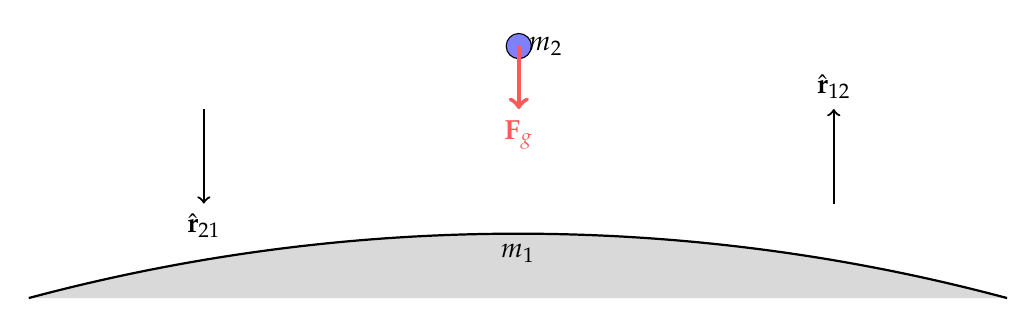
\begin{tikzpicture}[scale=0.8]
      \draw[thick,fill=gray!30] (7.75,0) arc(75:105:30)
      node[midway,below]{$m_1$};
      \draw[fill=blue!50] (0,4) circle(0.2) node[right]{$m_2$};
      \draw[ultra thick, red!65,->] (0,4)--(0,3)
      node[pos=1,below]{$\mb{F}_g$};
      \draw[->,thick](5,1.5)--(5,3) node[pos=1,above]{$\hat{\mb{r}}_{12}$};
      \draw[->,thick](-5,3)--(-5,1.5) node[pos=1,below]{$\hat{\mb{r}}_{21}$};
    \end{tikzpicture}
  \end{center}

  \vspace{-0.4in}{\Large
    \begin{displaymath}
      \boxed{
        \mb{F}_g
        =-\frac{Gm_1m_2}{r^2}\hat{\mb{r}}_{12}
        =+\frac{Gm_1m_2}{r^2}\hat{\mb{r}}_{21}
      }
    \end{displaymath}
  }

  where \fbox{$G=\SI{6.67e-11}{N.m^2/kg^2}$} is the universal gravitation
  constant, and $\hat{\mb{r}}_{12}$ and $\hat{\mb{r}}_{21}$ are
  \emph{unit vectors} (length=$1$)
\end{frame}


\begin{frame}
  \frametitle{Universal Gravitation}
  \begin{itemize}
  \item If $m_1$ exerts a gravitational force $\mb{F}_g$ on $m_2$, then $m_2$
    also exerts a gravitational force $-\mb{F}_g$ on $m_1$.
  \item The two forces are equal in magnitude and opposite in direction
    (Newton's 3rd law)
  \item Assumption: $m_1$ and $m_2$ are \emph{point masses}
    that do not occupy any space. We have already shown that the forces acting
    on an ensemble of masses is the same as acting at its center of mass
  \item Therefore, for the universal gravitational equation to work:
    
    \vspace{-0.2in}{\Large
      \begin{displaymath}
        r>(r_1+r_2)
      \end{displaymath}
    }
    That is, the two objects hasn't collided into one another
  \end{itemize}
\end{frame}


\section[$\mb{g}$]{Gravitational Field ($\mb{g}$)}


\begin{frame}
  \frametitle{Think Gravitational Field: What is $g$?}

  We generally describe the force of gravity as
  
  \vspace{-.25in}{\Large
    \begin{displaymath}
      \mb{F}_g=m\mb{g}
    \end{displaymath}
  }

  \vspace{-.2in}
  To find the magnitude of $g$, we group the variables in Newton's
  universal gravitation equation:
    
  \vspace{-.2in}{\Large
    \begin{displaymath}
      F_g=\underbrace{\left[\frac{Gm_1}{r^2}\right]}_{=g}m_2=m_2g
    \end{displaymath}
  }

  \vspace{-.1in}
  On the surface of Earth, we use use $m_1=m_\mathrm{Earth}$ and
  $r=r_\mathrm{Earth}$ to compute $g=\SI{9.81}{m/s^2}$, or $g=\SI{9.81}{N/kg}$
  (both units are  equivalent)
\end{frame}

\begin{frame}
  \frametitle{Gravitational Field}
  The intensity of the \textbf{gravitational field} $\mb{g}$ generated by
  a source mass $m_s$ is defined by:

  \vspace{-0.2in}{\Large
    \begin{displaymath}
      \boxed{g(m_s,r)=\frac{Gm_s}{r^2}}
    \end{displaymath}
  }
  
  It's a mapping of how $m_s$ influences the gravitational forces on other
  masses

  \begin{center}
    \begin{tabular}{l|c|c}
      \rowcolor{pink}
      \textbf{Quantity} & \textbf{Symbol} & \textbf{SI Unit} \\ \hline
      Gravitational field intensity    & $g$   & \si{N/kg}\\
      Universal gravitational constant & $G$   & \si{N.m^2/kg^2} \\
      Mass of source (a point mass)    & $m_s$ & \si{kg} \\
      Distance from centre of source   & $r$   & \si{m} \\
    \end{tabular}
  \end{center}
\end{frame}


\begin{frame}
  \frametitle{Relating Gravitational Field \& Gravitational Force}

  $\mb{g}$ itself doesn't do anything until there is another mass $m$. At which
  point, $m$ experiences a gravitational force  related to $\mb{g}$ by:

  \vspace{-0.2in}{\Large
    \begin{displaymath}
      \boxed{\mb{g}=\frac{\mb{F}_g}{m}}
    \end{displaymath}
  }
  
  $\mb{F}_g$ and  $\mb{g}$ are vectors in the same direction: toward the
  centre of the source mass that created the field, therefore all vector
  operations apply

  \begin{center}
    \begin{tabular}{l|c|c}
      \rowcolor{pink}
      \textbf{Quantity} & \textbf{Symbol} & \textbf{SI Unit} \\ \hline
      Gravitational field & $\mb{g}$   & \si{N/kg}\\
      Gravitational force on a mass & $\mb{F}_g$ & \si{N} \\
      Mass inside the gravitational field & $m$ & \si{kg} \\
    \end{tabular}
  \end{center}
\end{frame}



\begin{frame}
  \frametitle{What If You Are Inside Another Mass?}
  \framesubtitle{Case 1: A Spherical Shell of Radius $R$}

  \begin{columns}
    \column{0.3\textwidth}

    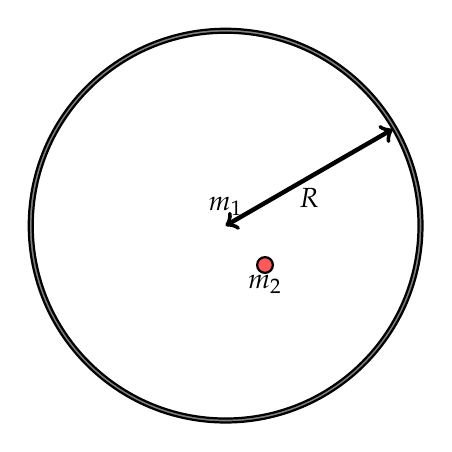
\begin{tikzpicture}[scale=0.5]
      \draw[thick,fill=gray](0,0) circle(5) node[above]{$m_1$};
      \draw[thick,fill=white](0,0) circle(4.9) node[above]{$m_1$};
      \draw[ultra thick,<->,rotate=30](0,0)--(4.9,0) node[midway,below]{$R$};
      \draw[thick,fill=red!65](1,-1) circle(0.2) node[below]{$m_2$};
    \end{tikzpicture}
    \column{0.7\textwidth}
    \begin{itemize}
    \item If a mass $m_2$ is \emph{inside} a spherical shell of mass $m_1$, the
      force of gravity it experiences is \textbf{zero}!
      
      \vspace{-.3in}{\Large
        \begin{displaymath}
          \boxed{
            \mb{F}_g=
            \begin{cases}
              \mb{0} & \text{if}\;\;r<R\\
              Gm_1m_2/r^2\hat{\mb{r}} & \text{otherwise}
            \end{cases}
          }
        \end{displaymath}
      }
      
    \item\vspace{-.2in} It also means that gravitational field is also
      \textbf{zero}
    \item There is a very similar case for a charged conducting sphere, where
      the electric field inside is also zero.
    \end{itemize}
  \end{columns}
\end{frame}



\begin{frame}
  \frametitle{What If You Are Inside Another Mass?}
  \framesubtitle{Case 2: Uniform Mass of Radius $R$}
  \begin{columns}
    \column{0.3\textwidth}

    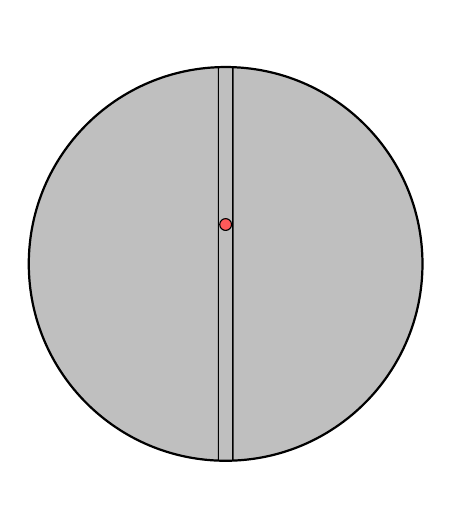
\begin{tikzpicture}[scale=0.5]
      \draw[thick,fill=gray!50](0,0) circle(5);
      \clip(-.2,-6) rectangle (.2,6);
      \draw[very thick](0.2,5)--(0.2,-5);
      \draw[very thick](-0.2,5)--(-0.2,-5);
      %\draw[ultra thick,<->,rotate=30](0,0)--(4.9,0) node[midway,below]{$R$};
      \draw[fill=red!65](0,1) circle(0.15) node[right]{$m_2$};
    \end{tikzpicture}
    \column{0.7\textwidth}

    \begin{center}
      \fbox{
        \begin{minipage}{.8\textwidth}
          Suppose you could drill a hole through the Earth and then drop into
          it. How long would it take you to pop up on the other side of the
          Earth?
        \end{minipage}
      }
    \end{center}
  \end{columns}
\end{frame}


\begin{frame}
  \frametitle{Falling To the Center of the Earth}
  Your initial gravitational force on the surface is:

  \vspace{-.2in}{\Large
    \begin{displaymath}
      F_g=mg_\mathrm{surface}\quad\quad\quad g_\mathrm{surface}=\SI{9.81}{N/kg}
    \end{displaymath}
  }

  \vspace{-.1in}
  $F_g$ becomes smaller as you approached the center, and when you reach
  the center, $F_g=0$.
  
  \vspace{.1in}
  Let's assume that the Earth is uniform density.
  We will also neglect air friction and other factors. Let's look at the value
  of $g$ as the person falls through Earth ($r<R$):

  \vspace{-.1in}{\Large
    \begin{displaymath}
      g(r)=\frac{GM(r)}{r^2}\quad M(r)=\frac{4}{3}\rho\pi r^3\quad
      \rho=\frac{3M_\mathrm{Earth}}{4\pi R^3}
    \end{displaymath}
  }
\end{frame}



\begin{frame}
  \frametitle{Falling To the Center of the Earth}

  \begin{columns}
    \column{0.25\textwidth}
    \pic{1}{eartholeg.png}
    \column{0.75\textwidth}
    Now we have an expression for the gravitational field strength inside
    ``Earth'':

    \vspace{-.2in}{\Large
      \begin{displaymath}
        g(r)=\frac{GM_\mathrm{Earth}r}{R^3}=g_\mathrm{surface}\frac{r}{R}
      \end{displaymath}
    }
    
    \vspace{-.1in}Gravitational field strength decreases linearly with $r$. At
    the center ($r=0$), $g=0$. Here's the interesting part, the gravitational
    force inside Earth is
    
    \vspace{-.3in}{\Large
      \begin{displaymath}
        F_g=-mg(r)=
        -\underbrace{\left[\frac{mg_\mathrm{surface}}{R}\right]}_{\textrm{constant}} r
        =-kr
      \end{displaymath}
    }
  \end{columns}
\end{frame}




\begin{frame}
  \frametitle{Falling To the Center of the Earth}

  \begin{columns}
    \column{0.25\textwidth}
    \pic{1}{eartholsat.png}
    \column{0.75\textwidth}
    So this poor guy is going to oscillate through Earth with a harmonic motion
    with a period of oscillation of:

    \vspace{-.2in}{\Large
      \begin{displaymath}
        T=2\pi\frac{m}{k}
      \end{displaymath}
    }

    which for Earth, is $T=\SI{5068}{\second}$. He
    would pop up on the opposite side after about
    \SI{42}{min}.

    \vspace{.1in}Suppose a satellite is in a circular orbit just above the
    surface, and passes overhead just above the traveler as he popped up
    out of the hole. The period of such an orbit would be the same as
    oscillating traveler.
    
  \end{columns}
\end{frame}



\section[$U_g$]{Gravitational Potential Energy ($U_g$)}


\begin{frame}
  \frametitle{Gravitational Potential Energy}

  \begin{itemize}
  \item The gravitational potential energy is defined as:
    {\Large
      \begin{displaymath}
        \boxed{U_g=-\frac{Gm_1m_2}{r}}
    \end{displaymath}
    }
  \item We can obtain this expression by integrating $\mb{F}_g$ by a distance
    $r$ to find the work done
  \item $U_g$ is the work required to move two objects from $r$ to $\infty$
  \item $U_g=0$ at $r=\infty$ and \emph{decrease} as $r$ decreases
  \end{itemize}
\end{frame}


\begin{frame}
  \frametitle{Relating Gravitational Potential Energy to Force}

  If you know vector calculus, you can easily see that gravitational
  force ($\mb{F}_g$) is the negative gradient of the gravitational potential
  energy ($U_g$):
  
  \vspace{-0.1in}{\Large
    \begin{displaymath}
      \mb{F}_g=-\nabla U_g=
      -\frac{\partial U_g}{\partial r}\hat{\mb{r}}
    \end{displaymath}
  }

  The direction of $\mb{F}_g$ always points from high to low potential
  \begin{itemize}
  \item A falling object is always decreasing in $U_g$
  \item ``Steepest descent'': the direction of $\mb{F}$ is the shortest path
    to decrease $U_g$ 
  \item Objects travelling perpendicular to $\mb{F}$ has constant $U_g$
  \end{itemize}
\end{frame}


\begin{frame}
  \frametitle{Relating $U_g$, $\mb{F}_g$ and $\mb{g}$}
  Knowing that $\mb{F}_g$ and $\mb{g}$ only differ by a constant, we can
  also relate gravitational field to $U_g$ by the gradient operator:

  \vspace{-0.1in}{\Large
    \begin{displaymath}
      \mb{g}=\frac{\mb{F}_g}{m}=-\nabla\left(\frac{U_g}{m}\right)=
      -\frac{\partial}{\partial r}\left(\frac{U_g}{m}\right)
      \hat{\mb{r}}
    \end{displaymath}
  }

  We already know that the direction of $\mb{g}$ is the same as $\mb{F}_g$,
  i.e.
  \begin{itemize}
  \item The direction of $\mb{g}$ is the shortest path to decrease $U_g$ 
  \item Objects travelling perpendicular to $\mb{g}$ has constant $U_g$
  \end{itemize}
\end{frame}


\begin{frame}
  \frametitle{Gravitational Field Lines}
  \begin{center}
    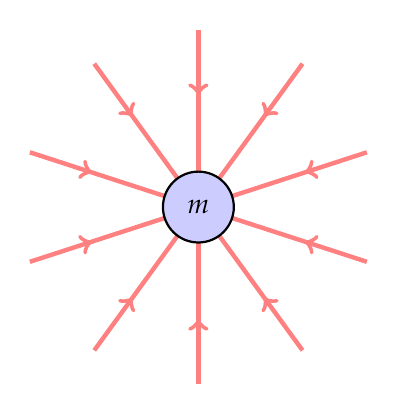
\begin{tikzpicture}[scale=1.5]
      \foreach \x in {0,...,9}\draw[red!50,ultra thick,rotate=36*\x](0,0)--(0,1);
      \foreach \x in {0,...,9}\draw[red!50,<-,ultra thick,rotate around={36*\x:(0,0)}](0,0.95)--(0,1.5);
      \draw[fill=blue!20,thick](0,0) circle(0.3) node{$m$};
    \end{tikzpicture}
  \end{center}
  \begin{itemize}
  \item The direction of $\mb{g}$ is towards the centre of the object that
    created it
  \item Field lines do not tell the intensity (i.e.\ magnitude) of $\mb{g}$,
    only the direction
  \end{itemize}
\end{frame}



\section{Orbits}

\begin{frame}
  \frametitle{Celestial Mechanics \& Kepler's Laws of Planetary Motion}
  In Physics 12, you studied briefly at the orbits of satellites around Earth,
  or the orbit of Earth and other planets around the Sun.
  \begin{itemize}
  \item Used your understanding of centripetal motion and gravity
  \item Assumed a circular orbit
  \end{itemize}
  Let's review some of those ideas.
\end{frame}


\begin{frame}
  \frametitle{Orbital Speed}
  \framesubtitle{Newton's Thought Experiment}
  \begin{center}
    \pic{1}{figure-5.jpg}
  \end{center}

  \vspace{-.3in}So how fast is fast enough?
\end{frame}


\begin{frame}
  \frametitle{Orbital Speed}
  \framesubtitle{Relating Gravitational and Centripetal Force}
  \begin{itemize}
  \item Assume a circular orbit (since we know it best)
  \item The centripetal force (required force) is equal to the gravitational
    force (supplied force):

    \vspace{-0.3in}{\Large
      \begin{displaymath}
        \underbrace{\frac{GMm}{r^2}}_\mathrm{F_g}
        =\underbrace{\frac{mv^2}{r}}_\mathrm{F_c}
      \end{displaymath}
    }
    where $r$ is the distance between the centres of the two objects
  \end{itemize}
\end{frame}



\begin{frame}
  \frametitle{Orbital Speed}
  \begin{itemize}
  \item Cancelling $m$, and $r$ in both sides of the equation, and solving for
    $v$, we get:
    
    \vspace{-0.15in}{\Large
      \begin{displaymath}
        \boxed{v_\mathrm{orbit}=\sqrt{\frac{GM}{r}}}
      \end{displaymath}
    }
  \item Orbital speed $v_\mathrm{orbit}$ is sometimes also called orbital
    velocity
  \item Does not depend on the mass of the object in orbit
  \item A $\SI{1.5e-13}{\kg}$ speck of cosmic dust and the $\SI{419600}{\kg}$
    International Space Station both have the same $v_\mathrm{orbit}$ around
    Earth if they are at the same altitude
  \end{itemize}
\end{frame}


\begin{frame}
  \frametitle{Escape Speed}
  An object can leave the surface of Earth at any speed. But when all the
  kinetic energy of that object is converted to gravitational potential, it'll
  return back to the surface of the earth. There is, however, a \emph{minimum}
  velocity at which the object \emph{would not} fall back to Earth because of
  gravity.
\end{frame}


\begin{frame}
  \frametitle{Escape Speed}
  \begin{itemize}
  \item The gravitational potential energy of an object with mass $m$ on the
    surface of a planet (with mass $M$ and radius $r$) is

    \vspace{-0.15in}{\Large
      \begin{displaymath}
        U_g=-\frac{GMm}{r}
      \end{displaymath}
    }
  \item The most amount of work that you can do is to bring it to the other side
    of the universe $r=\infty$, where $U_g=0$.
  \item If you start with \emph{more} kinetic energy than required to do all
    the work, then the object has \emph{escaped} the gravitational pull of the
    planet.
  \end{itemize}
\end{frame}


\begin{frame}
  \frametitle{Escape Speed}
  \begin{itemize}
  \item Set $K$ to equal to $-U_g$:
    
    \vspace{-0.2in}{\Large
      \begin{displaymath}
        \frac{1}{2}mv^2=\frac{GMm}{r}
      \end{displaymath}
    }
  \item We can then solve for escape speed $v=v_\mathrm{esc}$:

    \vspace{-0.2in}{\Large
      \begin{displaymath}
        \boxed{v_\mathrm{esc}=\sqrt{\frac{2GM}{r}}}
      \end{displaymath}
    }

  \item There is a simple relationship between orbital speed and escape
    speed:

    \vspace{-.2in}{\Large
      \begin{displaymath}
        \boxed{v_\mathrm{esc}=\sqrt{2} v_\mathrm{orbit}}
      \end{displaymath}
    }
  \end{itemize}
\end{frame}

\begin{frame}
  \frametitle{Example Problem}
  \textbf{Example:} Determine the escape velocity and energy for a
  \SI{1.60e4}{\kg} rocket leaving the surface of Earth.
\end{frame}

\begin{frame}
  \frametitle{What if I'm not escaping from the surface?}
  \begin{itemize}
  \item These two situations have the same escape speed:
    \begin{center}
      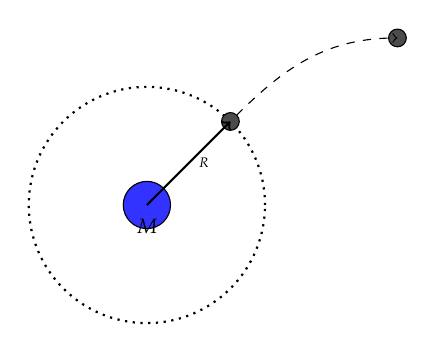
\begin{tikzpicture}[scale=1.5]
        \draw[fill=blue!80](0,0) circle(0.2) node[midway,below]{\tiny $M$};
        \draw[dotted,thick] (0,0) circle(1);
        \begin{scope}[rotate around={45:(0,0)}]
          \draw[fill=black!70](1,0) circle(0.075);
          \draw[->,thick](0,0)--(1,0) node[midway,right]{\tiny $R$};
          \draw[fill=black!70](2.5,-0.5) circle(0.075);
          \draw[->,dashed](1.075,0) to[out=0,in=135](2.5,-0.5);      
        \end{scope}
      \end{tikzpicture}
      \hspace{0.2in}
      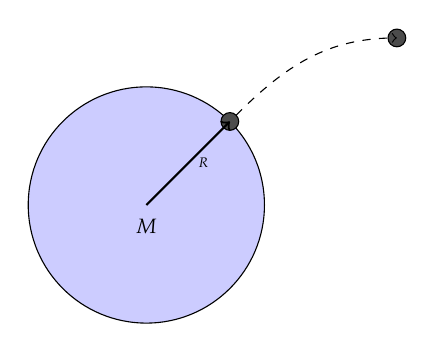
\begin{tikzpicture}[scale=1.5]
        \draw[fill=blue!20] (0,0) circle(1) node[midway,below]{\tiny $M$};
        \begin{scope}[rotate around={45:(0,0)}]
          \draw[fill=black!70](1,0) circle(0.075);
          \draw[->,thick](0,0)--(1,0) node[midway,right]{\tiny $R$};
          \draw[fill=black!70](2.5,-0.5) circle(0.075);
          \draw[->,dashed](1.075,0) to[out=0,in=135](2.5,-0.5);      
        \end{scope}
      \end{tikzpicture}
    \end{center}

  \item The only difference is that an object already in orbit (left figure)
    already has orbital speed $v_\mathrm{orbit}$, so escaping from that orbit
    requires an additional speed of

    \vspace{-0.45in}{\Large
      \begin{displaymath}
        \Delta v=v_\mathrm{esc}-v_\mathrm{orbit}
      \end{displaymath}
    }
  \end{itemize}
\end{frame}


\begin{frame}
  \frametitle{Orbital Energies}
  \begin{itemize}
  \item We can obtain the \textbf{orbital kinetic energy} by using the orbital
    speed in our expression of kinetic energy:

    \vspace{-.35in}{\Large
      \begin{displaymath}
        K_\mathrm{orbit}=\frac{1}{2}mv_\mathrm{orbit}^2=\frac{1}{2}m
        \left(\sqrt{\frac{GM}{r}}\right)^2=\boxed{\frac{GMm}{2r}}
      \end{displaymath}
    }
  \item And we already have an expression for
    \textbf{gravitational potential energy}:

    \vspace{-0.15in}{\Large
      \begin{displaymath}
        U_g=-\frac{GMm}{r}=-2K_\mathrm{orbit}
      \end{displaymath}
    }
  \item\textbf{Total orbital energy} is the sum of $K$ and $U_g$!

    \vspace{-0.15in}{\Large
      \begin{displaymath}
        E_T=K+U_g=-\frac{GMm}{2r}=-K_\mathrm{orbit}
      \end{displaymath}
      }
  \end{itemize}
\end{frame}





\section{Celestial Mechanics}


\begin{frame}
  \frametitle{Houston, We Have a Problem!}
  As always, this understanding isn't completely correct!
  \begin{itemize}
  \item Centripetal motion is based on rotation around a fixed point, but this
    is \emph{not} the case for celestial mechanics!
  \item Just as Earth orbits around the Sun, the Sun also experiences a
    centripetal force and therefore ``orbits'' around Earth
  \item This problem is especially important when the two objects orbiting each
    other has similar masses (e.g.\ a binary star system)
  \end{itemize}
\end{frame}


\begin{frame}
  \frametitle{Kepler's Laws of Planetary Motion}
  \begin{enumerate}
  \item\textbf{Law of Ellipses:} The orbit of a planet is an ellipse with the
    Sun at one of the two foci.
  \item\textbf{Law of Equal Areas:} A line segment joining a planet and the Sun
    sweeps out equal areas
  \item \textbf{Law of Periods:} The square of the orbital period of a planet
    is proportional to the cube of the semi-major axis of its orbit.
  \end{enumerate}
\end{frame}


\begin{frame}
  \frametitle{Kepler's Law of Planetary Motion}
  To fully understand Kepler's laws, we have to first understand the ellipse,
  at least a little bit.

  \begin{columns}
    \column{0.3\textwidth}
    \begin{center}
      \pic{1.25}{elliporb.png}
      
      $r' + r =2a$
    \end{center}
    \column{0.7\textwidth}
    \begin{itemize}
    \item The area of the ellipse is $A=\pi ab$
    \item The relationship between $r$ and $\theta$ given by:

      \vspace{-.3in}{\Large
        \begin{displaymath}
          r=\frac{a(1-e^2)}{1+e\cos\theta}
          \quad\textnormal{\footnotesize where}\quad
          0\leq e < 1
        \end{displaymath}
      }
    \item when $e=0$ it's a circle
    \item When $e=1$ it's no longer an ellipse
    \end{itemize}
  \end{columns}
\end{frame}


\begin{frame}
  \frametitle{Kepler's Law of Planetary Motion}
  \begin{columns}
    \column{0.6\textwidth}
    Most of the planets have very small eccentricity, so their orbits are
    fairly close to being circular, but comets are much more eccentric
    \column{0.4\textwidth}
    \begin{tabular}{l|l}
      \rowcolor{pink}
      \textbf{Object} & $e$ \\ \hline
      Mercury	& \num{0.206} \\
      Venus	& \num{0.0068} \\
      Earth	& \num{0.0167} \\
      Mars	& \num{0.0934} \\
      Jupiter	& \num{0.0485} \\
      Saturn	& \num{0.0556} \\
      Uranus	& \num{0.0472} \\
      Neptune	& \num{0.0086} \\
      Pluto	& \num{0.25} \\ \hline
      Halley's Comet   & \num{0.9671} \\
      Comet Hale-Bopp  & \num{0.9951} \\
      Comet Ikeya-Seki & \num{0.9999}
    \end{tabular}
  \end{columns}
\end{frame}

\begin{frame}
  \frametitle{Kepler's Law of Planetary Motion}
  \begin{center}
    \pic{.4}{kep5.png}
  \end{center}
\end{frame}



\begin{frame}
  \frametitle{Reduced Mass}

  Consider two objects orbiting each other. We know that the center of mass of
  the system is along the line between the two objects:
  \begin{center}
    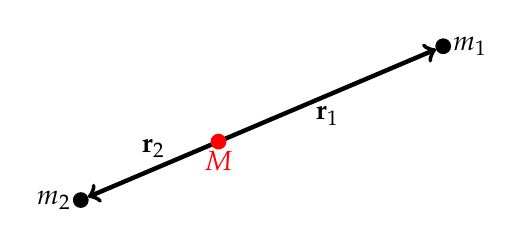
\begin{tikzpicture}
      \begin{scope}[rotate=23]
        \draw[ultra thick,->](0,0)--(3,0) node[midway,below]{$\mb{r}_1$};
        \draw[ultra thick,->](0,0)--(-1.8,0) node[midway,above]{$\mb{r}_2$};
        \fill[black] (3.1,0) circle(0.1) node[right]{$m_1$};
        \fill[black] (-1.9,0) circle(0.1) node[left]{$m_2$};
        \fill[red] (0,0) circle(0.1) node[below]{$M$};
      \end{scope}
    \end{tikzpicture}
  \end{center}

  \vspace{-.1in}
  The vectors $\mb{r}_1$ and $\mb{r}_2$ are relative to the center of mass, and
  the relative position $\mb{r}$ velocity $\mb{v}$ and acceleration $\mb{a}$
  between $m_1$ and $m_2$ are therefore:
  
  \vspace{-0.2in}{\Large
    \begin{displaymath}
      \mb{r}=\mb{r}_2 - \mb{r}_1\quad
      \mb{v}=\mb{v}_2 - \mb{v}_1\quad
      \mb{a}=\mb{a}_2 - \mb{a}_1
    \end{displaymath}
  }
\end{frame}



\begin{frame}
  \frametitle{Reduced Mass}
  
  From Newton's Third Law, we know that the gravitational force exerted by
  $m_1$ on $m_2$ is opposite the force exerted by $m_2$ on $m_1$:

  \vspace{-0.2in}{\Large
    \begin{displaymath}
      m_1\mb{a}_1+m_2\mb{a}_2=0
    \end{displaymath}
  }

  \vspace{-.2in}
  Substituting the expression for relative acceleration, now we have:

  \vspace{-0.2in}{\Large
    \begin{displaymath}
      \mb{a}=\mb{F}_g\left[\frac{1}{m_1}+\frac{1}{m_2}\right]=
      \mb{F}_g\left[\frac{m_1+m_2}{m_1m_2}\right]=\frac{\mb{F}_g}{\mu}
    \end{displaymath}
  }
  
  We can now define a new concept called \emph{reduced mass}:
  
  \vspace{-0.2in}{\Large
    \begin{displaymath}
      \mu=\frac{m_1m_2}{m_1+m_2}
    \end{displaymath}
  }
\end{frame}


\begin{frame}
  \frametitle{An Equivalent System}

  The orbit of one of the masses in a binary system is equivalent to the motion
  of the reduced mass orbiting around a point at relative distance $r$ where
  the total mass $M$ is placed. The magnitude of $r$ is the same as the
  relative distance $r$ in the development above.
  \begin{center}
    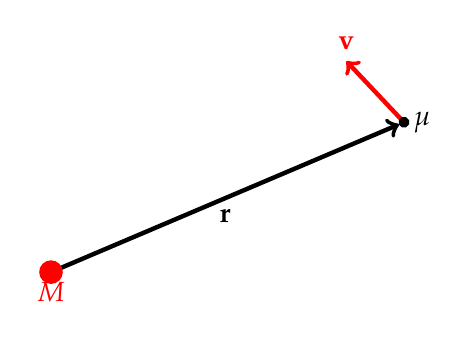
\begin{tikzpicture}
      \begin{scope}[rotate=23]
        \draw[ultra thick,->](0,0)--(4.8,0) node[midway,below]{$\mb{r}$};
        \draw[ultra thick,->,red](4.87,0)--(4.5,1) node[pos=1,above]{$\mb{v}$};
        \fill[red] (0,0) circle(0.15) node[below]{$M$};
        \fill[black] (4.87,0) circle(0.07) node[right]{$\mu$};
      \end{scope}
    \end{tikzpicture}
  \end{center}

  Both systems have the same total angular momentum.
\end{frame}



\begin{frame}
  \frametitle{Gravity is a Central Force}
  \begin{itemize}
  \item Gravity is called a \emph{central force} in that
  \item Gravitational force $\mb{F}_g$ is in the $-\hat{\mb{r}}$ direction, i.e.
    $\mb{F}\times\mb{r}=\mb{0}$
  \item Therefore gravity doesn't add torque
  \item No change in angular momentum: $\mb{L}=\textrm{constant}$
  \item This is true regardless of whether the orbit is circular or elliptical
  \end{itemize}
\end{frame}



\begin{frame}
  \frametitle{Now The Complicated Math}
  To show that the orbit is an ellipse (or it can be an ellipse), we need to
  show that the relationship between $r$ and $\theta$ is the one
  that we described earlier:

  \vspace{-0.15in}{\Large
    \begin{displaymath}
      r=\frac{a(1-e^2)}{1+e\cos\theta}
    \end{displaymath}
  } 
  
  The following steps will be shown \emph{only once}, and it's not important to
  be able to follow/remember everything here.
\end{frame}



\begin{frame}
  \frametitle{Complicated Calculations}
  The acceleration of the reduced mass:

  \vspace{-0.15in}{\Large
    \begin{displaymath}
      \mb{a}=-\frac{GM}{r^2}\hat{\mb{r}}
    \end{displaymath}
  }

  To find the expression for $r$, we first do a cross product of $\mb{a}$ with
  $\mb{L}$:
  
  \vspace{-0.3in}{\Large
    \begin{displaymath}
      \mb{a}\times\mb{L}=-\frac{GM}{r^2}\hat{\mb{r}}\times
      \left(\mu r^2\hat{\mb{r}}\times\frac{d\hat{\mb{r}}}{dt} \right)
      =GM\mu\hat{\mb{r}}\times
      \left(\hat{\mb{r}}\times\frac{d\hat{\mb{r}}}{dt} \right)
    \end{displaymath}
  }
  We then apply the vector identity
  $\mb{A}\times(\mb{B}\times\mb{C})=(\mb{A}\cdot\mb{C})\mb{B}-(\mb{A}\cdot\mb{B})\mb{C}$ and the expression magically reduces to:

  \vspace{-0.3in}{\Large
    \begin{displaymath}
      \mb{a}\times\mb{L}=GM\mu\frac{d\hat{\mb{r}}}{dt}
    \end{displaymath}
  }
\end{frame}



\begin{frame}
  \frametitle{Confused Yet?}
  Now we move on to another expression that is closer to where we need to be:

  \vspace{-0.25in}{\Large
    \begin{displaymath}
      \frac{d}{dt}\left(\mb{v}\times\mb{L}\right)=
      \frac{d\mb{v}}{dt}\times\mb{L} +
      \mb{v}\times \cancel{\frac{d\mb{L}}{dt}}=\mb{a}\times\mb{L}
      =\frac{d}{dt}\left(GM\mu\hat{\mb{r}}\right)
    \end{displaymath}
  }

  Integrating both sides with respect to $t$ and we get:

  \vspace{-0.2in}{\Large
    \begin{displaymath}
      \mb{v}\times\mb{L}=GM\mu\hat{\mb{r}} +\mb{D}
    \end{displaymath}
  }
  where $\mb{D}$ is some constant of integration. Now we take the dot product
  with $\mb{r}$

  \vspace{-0.2in}{\Large
    \begin{displaymath}
      \mb{r}\cdot\left(\mb{v}\times\mb{L}\right)
      =GM\mu r + \mb{r}\cdot\mb{D}
    \end{displaymath}
  }
\end{frame}



\begin{frame}
  \frametitle{Just One More Slide!}
  We once again apply some vector identity:
  $\mb{A}\cdot(\mb{B}\times\mb{C})=(\mb{A}\times\mb{B})\cdot\mb{C}$ and we
  get:

  \vspace{-0.3in}{\Large
    \begin{displaymath}
      \left(\mb{r}\times\mb{v}\right)\cdot\mb{L}
      =GM\mu r + rD\cos\theta
    \end{displaymath}
  }

  \vspace{-.2in}
  The final step is to recognize that if we define $e=D/GM\mu$, then we can 
  express $r$ as:
  
  \vspace{-0.3in}{\Large
    \begin{displaymath}
      r=\frac{L^2/\mu^2}{GM(1+e\cos\theta)}
    \end{displaymath}
  }
  
  This is an expression for an ellipse!
    
  \vspace{-.2in}{\Large
    \begin{displaymath}
      r=\frac{a(1-e^2)}{1+e\cos\theta}\quad\textnormal{if}\quad
      L=\mu\sqrt{GMa(1-e^2)}
    \end{displaymath}
  }  
\end{frame}


\begin{frame}
  \frametitle{Kepler's First Law: Law of Orbits}
  \begin{columns}
    \column{.3\textwidth}
    \vspace{0.2in}
    \pic{1.2}{kepo17.png}
    \column{.7\textwidth}
    \begin{center}
      \fbox{
        \begin{minipage}{.85\textwidth}
          For a bound binary orbit, each object will follow an elliptical orbit
          about the center of mass of the system. The center of mass will be at
          one focus of each ellipse
        \end{minipage}
      }
    \end{center}
    \begin{itemize}
    \item This is of course \emph{slightly} different from Kepler's conclusion!
    \item But if one of the mass is very large compared to the other one,
      i.e.\ $m_1\gg m_2$, then the center of gravity is essentially at $m_1$
      and $m_2$ is orbiting around $m_1$ in an ellipse
    \end{itemize}
  \end{columns}
\end{frame}



\begin{frame}
  \frametitle{Kepler's 2nd Law: The Law of Equal Areas}

  \vspace{0.2in}
  \begin{center}
    \fbox{
      \begin{minipage}{0.9\textwidth}
      \textbf{Second Law: A line segment joining a planet and the Sun sweeps
        out equal areas during equal intervals of time}
      \end{minipage}
    }

    \pic{.6}{201532-132212364-3243-planet.jpg}
  \end{center}
\end{frame}


\begin{frame}
  \frametitle{Kepler's 2nd Law: The Law of Equal Areas}
  \begin{center}
    \fbox{
      \begin{minipage}{0.9\textwidth}
      \textbf{Second Law: A line segment joining a planet and the Sun sweeps
        out equal areas during equal intervals of time}
      \end{minipage}
    }
  \end{center}

  \begin{columns}
    \column{.25\textwidth}
    \pic{1.2}{kepa1.png}
    \column{.75\textwidth}
    \begin{itemize}
    \item The infinitesimal area swept out by an object in orbit is given by
      
      \vspace{-.3in}{\Large
        \begin{displaymath}
          dA=\frac{1}{2}r^2d\theta
        \end{displaymath}
      }
    \item Take the time derivative of both sides, and we have an expression for
      \emph{areal velocity} (yes, that's a real word in celestial mechanics):
      
      \vspace{-.2in}{\Large
        \begin{displaymath}
          \frac{dA}{dt}=\frac{1}{2}r^2\frac{d\theta}{dt}=\frac{1}{2}r^2\omega
        \end{displaymath}
      }
    \end{itemize}
  \end{columns}
\end{frame}


\begin{frame}
  \frametitle{Kepler's 2nd Law: The Law of Equal Areas}

  \begin{itemize}
  \item But hurray! We know that the angular component of velocity
    ($\mb{v}_\theta$) is related to the angular velocity $\mb{\omega}$, so:
    
    \vspace{-.25in}{\Large
      \begin{displaymath}
        v_\theta=r\omega\quad\longrightarrow\quad
        \frac{dA}{dt}
        =\frac{1}{2}r(r\omega)
        =\frac{1}{2}rv_\theta
      \end{displaymath}
    }
  \item Hurray again! Because we know that
    
    \vspace{-.4in}{\Large
      \begin{displaymath}
        rv_\theta=|\mb{r}\times\mb{v}_\theta|=|\frac{\mb{L}}{\mu}|=\frac{L}{\mu}
        \quad\longrightarrow\quad
        \boxed{\frac{dA}{dt} =\frac{L}{2\mu}}
      \end{displaymath}
    }
  \item Since we know that angular momentum is conserved (i.e. $L$ is constant),
    areal velocity is a constant, therefore it sweeps out equal areas in equal
    intervals of time
  \end{itemize}
\end{frame}


\begin{frame}
  \frametitle{Kepler's Third Law: The Law of Periods}
  \begin{center}
    \fbox{
      \begin{minipage}{0.9\textwidth}
        \textbf{Law of Periods: The square of the orbital period of a planet
          is proportional to the cube of the semi-major axis of its orbit.}
      \end{minipage}
    }
  \end{center}
\end{frame}

\begin{frame}
  \frametitle{Kepler's Third Law: The Law of Periods}
  \begin{itemize}
  \item Now that we have an expression for areal velocity (a constant!), we can
    integrate with respect to time, from $t=0$ to $t=T$ to get the period:

    \vspace{-.2in}{\Large
      \begin{displaymath}
        \int_0^T\frac{dA}{dt}dt=\frac{L}{2\mu}\int_0^Tdt
        \quad\longrightarrow\quad
      A=\frac{L}{2\mu}T
      \end{displaymath}
    }
  \item But we know that the area of an ellipse is given by:

    \vspace{-.2in}{\Large
      \begin{displaymath}
        A=\pi ab\quad\quad\textnormal{and}\quad\quad b^2=a^2(1-e^2)
      \end{displaymath}
    }
    where $e$ is the eccentricity of the ellipse
  \item Combine that also with the expression for angular momentum:

    \vspace{-.2in}{\Large
      \begin{displaymath}
        L=\mu\sqrt{GMa(1-e^2)}
      \end{displaymath}
    }
    where $M$ is the total mass of the two celestial objects

  \end{itemize}
\end{frame}


\begin{frame}
  \frametitle{Kepler's Third Law: The Law of Periods}
  \begin{itemize}
  \item After some algebra, we end up with this equation

    \vspace{-.2in}{\Large
      \begin{displaymath}
        \boxed{T^2
          =\underbrace{\left[\frac{4\pi^2}{GM}\right]}_{\textrm{constant}} a^3
        }
      \end{displaymath}
    }

  \item Remember that $M$ is the total mass of the two objects. For the case
    where one object (e.g.\ sun) is much more massive than the other (e.g.\
    Earth), i.e.\ $m_1\gg m_2$, we can just use $M\approx m_1$

  \end{itemize}
\end{frame}



\begin{frame}
  \frametitle{Kepler's Third Law: The Law of Periods}
  \begin{center}
    \pic{.65}{kep8.png}
  \end{center}
\end{frame}

\end{document}
